\subsection{Unsicherheiten}\label{subsec:unc}

	Jegliche Unsicherheiten werden nach GUM bestimmt und berechnet.
	Die Gleichungen dazu finden sich in Gl. \ref{fig:GUM_combine} und Gl. \ref{fig:GUM_formula}.
	Für die Unsicherheitsrechnungen wurde die Python Bibliothek "uncertainties" herangezogen, welche den Richtlinien des GUM folgt.
	Alle konkreten Unsicherheitsformeln stehen weiter unten.
	Für Unsicherheiten in graphischen Fits wurden die $y$-Unsicherheiten beachtet und die Methode der kleinsten Quadrate angewandt.
	Dafür steht in der Bibliothek die Methode "scipy.optimize.curve\_fit()" zur Verfügung.
	
	Für digitale Messungen wird eine Unsicherheit von $u(X) = \frac{\Delta X}{2\sqrt{3}}$ angenommen, bei analogen eine von $u(X) = \frac{\Delta X}{2\sqrt{6}}$.
	
	\vspace{1,5cm}	
	\begin{equation} \label{fig:GUM_combine}	
		x = \sum_{i=1}^{N} x_i
		;\quad
		u(x) = \sqrt{\sum_{i = 1}^{N} u(x_i)^2}		
	\end{equation}
	\begin{center}
		{Formel für kombinierte Unsicherheiten des selben Typs nach GUM.}
	\end{center}
			
	\begin{align} \label{fig:GUM_formula}
		f = f(x_1, \dots , x_N)
		;\quad
		u(f) = \sqrt{\sum_{i = 1}^{N}\left(\pdv{f}{x_i} u(x_i)\right) ^2}
	\end{align}
	\begin{center}
		{Formel für sich fortpflanzende Unsicherheiten nach GUM.}	
	\end{center}
	
	\vspace{1cm}	
	\begin{flushleft}
		\textbf{Weitere Unsicherheiten:}
	\end{flushleft}	
	\begin{description}
	
		\item[Millimeter pro 16 Pixel] Für die Millimeter pro 16 Pixel wurde eine Unsicherheit von $u(\text{Skalierung}) = \SI{0,05}{\milli\meter}$ gewählt.
		\item[Schräge Skala $d$] Für die Unsicherheit bei dem Ablesen der Skala auf dem schrägen Schirm wurde eine größere Unsicherheit von $ u(d) = \SI{5}{\milli\meter}$ gewählt, da der genaue Punkt des Übergangs zwischen scharf und unscharf nicht eindeutig zu bestimmen war.
		\item[Höhe des scharfen Bereichs $h$] Analog zu der schrägen Skala wird hier eine große Unsicherheit angenommen, hier $ u(h) = \SI{2,5}{\milli\meter}$.
		\item[Subjektive Schärfentiefe $S_\text{sub}$] Diese Unsicherheit folgt aus letzteren und Gl. \ref{fig:GUM_combine}.
		Sie wird durch 
		\begin{align}
			S_\text{sub} &= \sqrt{d^2-h^2} \\
			\rightarrow u(S_\text{sub}) &= \sqrt{\left( \frac{d\cdot u(d)}{\sqrt{d^2-h^2}}\right)^2 + \left( \frac{- h\cdot u(h)}{\sqrt{d^2-h^2}}\right)^2} 
		\end{align}
		\item[hyperfokale Entfernung $d_\text{h}$] Da Brennweite $f$ und Blendenzahl $k$ hierbei als absolut angesehen werden, trägt nur die Unsicherheit der Bilddiagonalen $D_\text{B}$ zu der Unsicherheit der hyperfokalen Entfernung bei:
		\begin{align}
			d_\text{h} &= \frac{f^2}{k\cdot Z} + f = \frac{1500\cdot f^2}{k\cdot D_\text{B}} + f \\
			\rightarrow u(d_\text{h}) &= \frac{1500\cdot f^2}{k\cdot D_\text{B}^2} \cdot u(D_\text{B})
		\end{align}	
		\item[Gegenstandsweite $g$] Diese Größe wurde mit einem Maßband gemessen. Da, wegen des Objektivs, nicht genau von der Linse bis zu dem Schirm gemessen werden konnte, wurde hier eine größere Unsicherheit als bei einer Dreiecksverteilung von $u(g) = \SI{10}{\milli\meter}$ angenommen.
		\item[theoretische Schärfentiefe] Diese Unsicherheit setzt sich aus denen der Gegenstandsweite $g$ und der hyperfokalen Entfernung $d_\text{h}$ zusammen, welche aus den Gleichungen für Nahpunkt $d_\text{n}$ und Fernpunkt $d_\text{f}$ stammen.
		\begin{align}
			S = d_\text{f} - d_\text{n} &= g\cdot (d_\text{h}-f) \cdot \left( \frac{1}{d_\text{h} - g} - \frac{1}{d_\text{h} + g -2f} \right) \\
			\frac{\dd S}{\dd d_\text{h}} &= \frac{g}{d_\text{h} - g} - \frac{(d_\text{h} - f)\cdot g}{(d_\text{h} - g)^2} + \frac{g}{d_\text{h} + g - 2f} + \frac{(d_\text{h} - f)\cdot g}{(d_\text{h} + g - 2f)^2} \\
			\frac{\dd S}{\dd g} &= \frac{(d_\text{h} - f)}{d_\text{h} - g} + \frac{(d_\text{h} - f)\cdot g}{(d_\text{h} - g)^2} - \frac{(d_\text{h} - f)}{d_\text{h} + g - 2f} + \frac{(d_\text{h} - f)\cdot g}{(d_\text{h} + g - 2f)^2} \\
			\rightarrow u(S) &= \sqrt{\left( \frac{\dd S}{\dd d_\text{h}} \cdot u(d_\text{h}) \right)^2 + \left( \frac{\dd S}{\dd g} \cdot u(g) \right)^2 }
		\end{align}
	
		\item[Siemenssterne] Aus der Bedrachtung der Siemenssterne ist die Auflösung der Linienbreite 
		\begin{equation}
			A = \frac{\pi }{36} h; \quad u(A) = \frac{\pi}{36} u(h),
		\end{equation}
		wobei $h$ die Halbwertsbreite der Grauwertdifferenz ist.
		
		\item[Graustufen] Angeben auf einer Grauskala von $0$ bis $255$ wurden mit $Delta = 5$ betrachtet.
		
		\item[Belichtungszeit] Die Kamera hat keine expliziten Daten angegeben.
		Es wurde $\Delta T = 0,01 T$ angenommen.
		
	\end{description}

\newpage
\subsection{Zusatzbilder}\label{subsec:Zusatz}

\begin{figure}[ht]
	\centering
	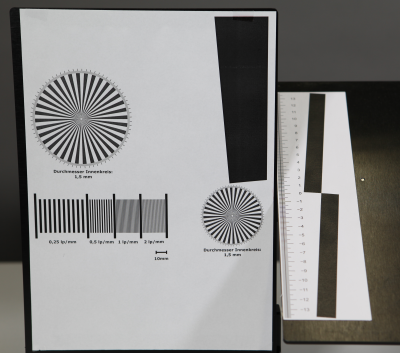
\includegraphics[width=0.55\textwidth]{bilder/testbild.png}
	\caption{Testbild.\cite{WWU}}
	\label{fig:testbild}	
\end{figure}	


\begin{figure}[ht]
	\centering
	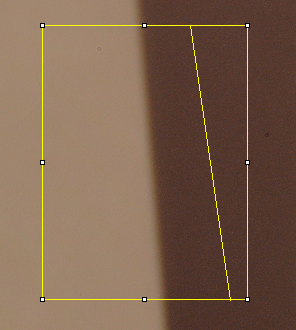
\includegraphics[width=0.30\textwidth]{bilder/MTF-Fehler.PNG}
	\caption{Fehler bei dem ImageJ-Plugin.}
	\label{fig:fail}	
\end{figure}